%%%%%%%%%%%%%%%%%%%%%%%%%%%%%%%%%%%%%%%%%%%%%%%%%%%%%%%%%%%%%%%%%%%%%%%%%%%%%%%%%%%%%%%%%%%%%%%%%%%%%
%%%%%%%%%%%%%%%PART-B(Question#04--> 
%%%%%%%%%%%%%%%%%%%%%%%%%%%%%%%%%%%%%%%%%%%%%%%%%%%%%%%%%%%%%%%
%%%%%%%%%%%%%%%%%%%%%%%%%%%%%%%%%%%%%%%%%%%%%%%%%%%%%%%%%%%%%%%%%%%%%%%%%%%%%%%%	
\question 
\begin{parts} 
%%%%%%%%%%%%%%%%%%%%%%%%%%%%%%%%%%%%%%%%%%%%%%%%%%%%%%%%%%%%%%%%%	
\part[6] An Inverse Definite Minimum Time (IDMT) overcurrent relay is connected to a \qty[parse-numbers=false]{400/5}{\ampere} Current Transformer (CT) with a Plug Setting (PS) of $125\%$. The characteristic curve for $\text{TMS} = 1.0$ is shown in Fig.~\ref{fig:graph}. If a symmetrical fault current of \qty{5000}{\ampere} flows through the primary side, calculate:

\begin{subparts}
    \subpart The Plug Setting Multiplier ($\text{PSM}$) of the relay.
    \subpart The operating time of the relay for $\text{TMS} = 0.4$.
    \subpart The required $\text{TMS}$ setting if the relay must operate in $1.8\text{ seconds}$.
\end{subparts}


\begin{figure}[H]
\centering
\resizebox{0.5\textwidth}{!}{% Adjust width (e.g., 0.6\textwidth, 10cm, etc.) as needed
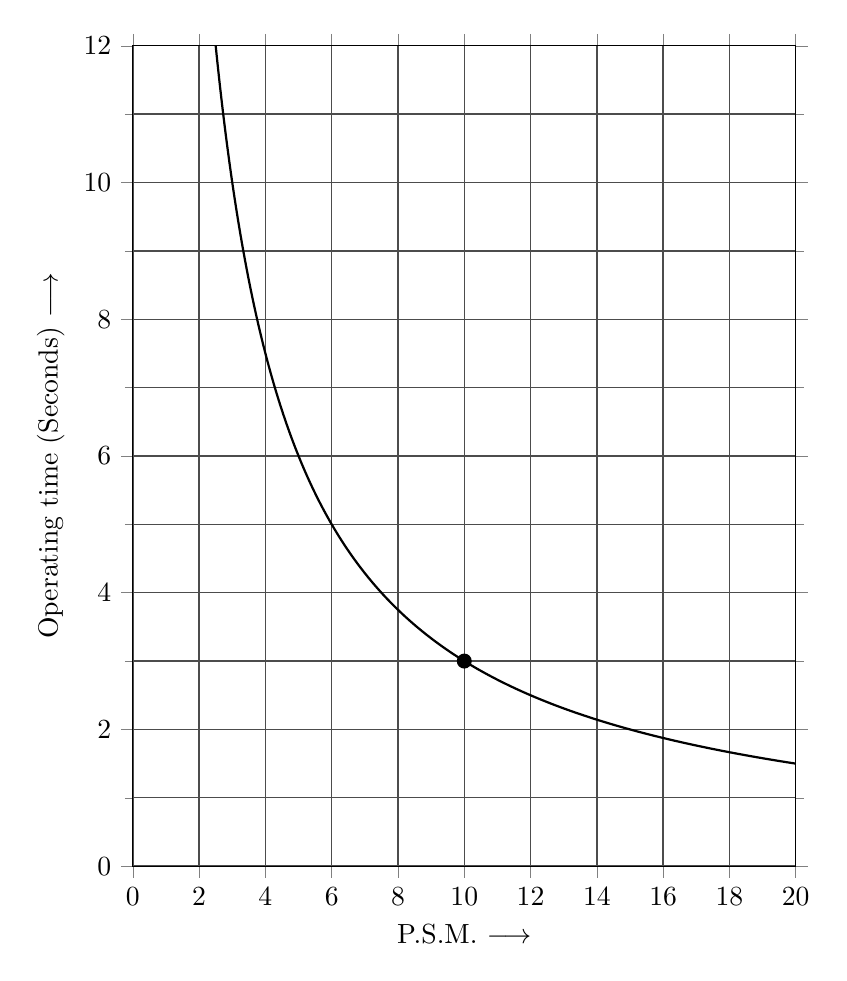
\begin{tikzpicture}
\begin{axis}[
    width=10cm,
    height=12cm,
    xmin=0, xmax=20,
    ymin=0, ymax=12,
    % Horizontal labels at 0, 2, 4... 20
    xtick={0,2,4,6,8,10,12,14,16,18,20},
    % Vertical labels at 0, 2, 4... 12
    ytick={0,2,4,6,8,10,12},
    % NO extra vertical lines (only at the 2-unit marks)
    minor x tick num=0,
    % EXTRA horizontal lines (adds 1 line between the 2-unit marks)
    minor y tick num=1,
    % Grid settings
    grid=both,
    % Make all grid lines look the same to match the photo
    grid style={line width=0.5pt, draw=black!70},
    % Axis labels
    xlabel={P.S.M. $\longrightarrow$},
    ylabel={Operating time (Seconds) $\longrightarrow$},
    % Visual formatting
    tick align=outside,
    axis lines=box,
    enlargelimits=false,
    samples=200
]

% The IDMT characteristic curve function
\addplot[
    domain=2.1:20, 
    smooth, 
    thick, 
    black
] {30/x}; 

% The dot at PSM=10, Time=3
\addplot[only marks, mark=*, mark size=2.5pt] coordinates {(10,3)};

\end{axis}
\end{tikzpicture}%
}
\caption{IDMT Overcurrent Relay Characteristic Curve}
\label{fig:graph}
\end{figure}



\begin{solution}
\textbf{(a) Plug Setting Multiplier ($\text{PSM}$):}
$$\text{Pick-up Current} = I_{\text{pickup}} = 5\text{ A} \times 1.25 = 6.25\text{ A}$$
$$\text{Secondary Fault Current} = I_{\text{sec}} = 5000\text{ A} \times \left(\frac{5}{400}\right) = 62.5\text{ A}$$
$$\text{PSM} = \frac{I_{\text{sec}}}{I_{\text{pickup}}} = \frac{62.5\text{ A}}{6.25\text{ A}} = 10$$

\textbf{(b) Operating time for $\text{TMS} = 0.4$:}
From Fig.~\ref{fig:graph}, at $\text{PSM} = 10$, the operating time at $\text{TMS} = 1.0$ is $t_{1.0} = 3.0\text{ s}$.
$$t = t_{1.0} \times \text{TMS} = 3.0\text{ s} \times 0.4 = 1.2\text{ s}$$

\textbf{(c) Required $\text{TMS}$ for $t = 1.8\text{ s}$:}
$$\text{TMS} = \frac{t}{t_{1.0}} = \frac{1.8\text{ s}}{3.0\text{ s}} = 0.6$$
\end{solution}
%%%%%%%%%%%%%%%%%%%%%%%%%%%%%%%%%%%%%%%%%%%%%%%%%%%%%%%%%%%%%%%%%		
\part[4]For the emitter bias network of Fig.~\ref{fig:ckt-bjt-emitter-bias} determine \(I_{B}\), \(I_{C}\), \(V_{CE}\), \(V_C\), \(V_E\) and \(V_B\).

\begin{figure}[H]
\centering
\resizebox{0.6\textwidth}{!}{% Adjust width (e.g., 0.6\textwidth, 10cm, etc.) as needed
\begin{tikzpicture}
	% Paths, nodes and wires:
	\draw node[npn] (N1) at (6, 4) {} node[anchor=west] at ([xshift=0.88cm]N1.east){$\beta = 50$};
	\draw (6, 7) to[american resistor, l={$2~k\Omega$}, label distance=0.02cm] (6, 4.77);
	\draw (5.16, 4) -- (2, 4);
	\draw (3, 7) to[american resistor, l_={$430~k\Omega$}, label distance=0.02cm] (3, 4);
	\draw (3, 7) -- (6, 7);
	\draw node[circ] at (4.51, 7) {};
	\draw (4.5, 7) -| (4.5, 7.5);
	\draw node[ocirc] (N2) at (4.5, 7.5) {} node[anchor=south] at (N2.north){$ +20~V$};
	\draw (7.316, 4.77) to[curved capacitor, l={$10~\mu F$}, label distance=0.02cm] (10.316, 4.8);
	\draw (2, 4) to[curved capacitor, l_={$10~\mu F$}, label distance=0.02cm] (0, 4);
	\draw node[ocirc] (N3) at (0, 4) {} node[anchor=east] at (N3.west){$v_i$};
	\draw node[ocirc] (N4) at (10.316, 4.8) {} node[anchor=west] at (N4.east){$v_o$};
	\draw (6, 4.77) -- (7.316, 4.77);
	\draw node[circ] at (3, 4) {};
	\draw node[circ, xscale=1.13, yscale=1.13] at (6, 4.77) {};
	\draw (6, 3.23) to[american resistor, l={$1~k\Omega$}, label distance=0.02cm] (6, 1);
	\draw (8, 2.5) to[capacitor, l={$40~\mu F$}, label distance=0.02cm] (8, 1);
	\draw (6, 3.23) -| (8, 2.5);
	\draw node[tlground] at (6, 1) {};
	\draw node[tlground] at (6, 1) {};
	\draw node[tlground] at (8, 1) {};
	\draw node[tlground] at (8, 1) {};
	\draw node[circ] at (6, 3.23) {};
\end{tikzpicture}
}
\caption{}
\label{fig:ckt-bjt-emitter-bias}

\end{figure}


\begin{solution}


\end{solution}
%%%%%%%%%%%%%%%%%%%%%%%%%%%%%%%%%%%%%%%%%%%%%%%%%%%%%%%%%%%%%%%%%	
\end{parts}
